%Preamble
\documentclass[12pt]{article}
\usepackage{preprint}
\usepackage{authblk}
\usepackage[utf8]{inputenc}
\usepackage[T1]{fontenc}
\usepackage{amsmath}
\usepackage{amssymb}
\usepackage{amsthm}
\usepackage{amsrefs}
\usepackage{amsfonts}
\usepackage{mathrsfs}
\usepackage{mathtools}
\usepackage{enumerate}
\usepackage[shortlabels]{enumitem}
\usepackage{verbatim} %% includes comment environment
\usepackage{hyperref}
\usepackage[capitalize]{cleveref}
\crefformat{equation}{~(#2#1#3)}
\usepackage{caption, subcaption}
\usepackage{graphicx}
\usepackage{fullpage} %%smaller margins
\usepackage{mathrsfs}
\usepackage{lineno}
\linenumbers

\renewcommand{\vec}[1]{\boldsymbol{#1}}

\linespread{1.5} % Increase Line spread

\title{SARS-CoV-2 variant dynamics across US states show consistent differences in effective reproduction numbers}

\author[1,2,*]{Marlin D.\ Figgins}
\author[1,3]{Trevor Bedford}
\affil[1]{Vaccine and Infectious Disease Division, Fred Hutchinson Cancer Research Center, Seattle, WA, USA}
\affil[2]{Department of Applied Mathematics, University of Washington, Seattle, WA, USA}
\affil[3]{Howard Hughes Medical Institute, Seattle, WA, USA}
\affil[*]{Corresponding author: mfiggins@uw.edu}
\date{\today}
%Figure out author affilations...
% https://maehler.se/blog/2013/11/01/authors-and-affiliations-in-latex

\begin{document}

%TODO: Be consistent on the language of lineage v. variant
%TODO: Focus on synthesizing literature in the discussion to discuss limitations and future directions
%TODO: What should two sentence takeaway be if I had to explan this to someone who was familiar with this line of work?

\maketitle

\begin{abstract}
Reconciling genetic data of SARS-CoV-2 lineages with epidemic surveillance data is difficult.
Models of infectious diseases using genomic data typically rely on phylogenetic and phylodynamic inference which have issues scaling to large number of samples. %TODO: Do we have an upper bound here?
In response to this, recent studies have used the sample proportions of different variants as an approximation to the variant frequencies and to describe variant frequency dynamics, but frequencies alone cannot capture the rich epidemiological behavior of SARS-CoV-2.
We extend methods for inferring the effective reproduction number of an epidemic using confirmed case data to jointly estimate variant-specific effective reproduction numbers and frequencies of several co-circulating SARS-CoV-2 variants using case data and genetic sequences across states in the US from January to October 2021.
Our method can be used to infer structured relationships between effective reproduction numbers across time series which may be amendable to various analyses including other features related to the effective reproductive number such as non-pharmaceutical interventions.
We use this model to quantify growth advantages for various SARS-CoV-2 Variants of Concern and Variants of Interest in the United States and estimate the effect of vaccination on curbing the spread of different variants in the United States.
%TODO: Sentence about growth advantages
%TODO: Sentence about the applicability of this method generally
\end{abstract}

\section{Introduction}%

%TODO: Lead into the pandemic, thorough descriptions on how genetic differences in variants may lead to different outcomes at the level of transmission and clinical presentation.
%TODO: Move into the specifics of SARS-CoV-2. What info does a reader 2 years from now need to know to be able to make sense of this work?
%TODO: Mention that modeling efforts are useful for understanding what has happened over the course of the pandemic.
%TODO: And will be useful for tackling the continued spread of SARS-CoV-2

As SARS-CoV-2 evolves, extant lineages may increase in their ability to transmit and escape acquired immunity \cite{Tegally2020}. %TODO: MF Expand slightly.  %TODO: Reference here TB: Cite canonical B.1.1.7 paper and canonical B.351.1 paper. MF: Which B.1.1.7 paper, did you mean?
Quantifying the observed growth advantages of SARS-CoV-2 variants of concern allow us to understand which variants are able to thrive in different locations.
%TODO: Mention that GISAID exists and is relevant here.
Relating genomic data of SARS-CoV-2 lineages to epidemic surveillance data is difficult.
Though it is typical to use phylodynamic methods to analyze genetic sequence data from epidemics, the sheer amount of data ([NUM OF SEQUENCES AS OF DATE]) makes these methods hard to use at the scale of interest due to computational constraints associated with the large numbers of sequences.
In order to deal with the limitations of phylodynamic inference in this large sample size regime, previous studies have estimated the growth of lineages using observed frequencies in sequenced SARS-CoV-2 samples \cites{Annavajhala2021, Faria2021, Obermeyer2021, Ito2021}. %TODO: Cite papers here? TB: There are some early B.1.1.7 papers worth citing. A self-cite of Annavajhala et al would also work in this context.
These methods often model the frequency of lineages using multinomial logistic regression. \cites{Ito2021, Obermeyer2021}
These methods have the advantage of being more scalable with increased sampling rate as individual sequences are reduced to a count of each lineage for each day, but they do not directly account for the complicated infection and transmission dynamics which influence which lineages succeed and are observed in real life.
Growth of frequencies alone cannot capture the rich epidemiological behavior of SARS-CoV-2 variant transmission.
When dealing with competition between variants, variants which are declining in frequency can still lead to an increasing number of infections.
Similarly, growth in frequency does not necessarily entail an increase in absolute infections.
%TB: I find the "limitations of phylodynamic inference" aspect to be a bit of a distraction. Phylodynamic methods are actually quite poor at estimating fitnesses of different clades and are usually used for things like prevalence via skyline plots or geographic spread via phylogeography. So it's not just dataset size but a more foundemental lack of appropriate methods.

To better capture epidemiological dynamics, there are methods which describe the growth of total infections using confirmed case, hospitalization, or death data to estimate changes in the effective reproduction number $R_{t}$, the average number of infections a single infectious individual generates, during a given outbreak.
Though, these methods are excellent for describing overall growth rates, they cannot capture the evolutionary dynamics and fitness changes between different variants since they often assume the population dynamics are described by a singular $R_{t}$ trajectory. \cites{Cori2013, Abbott2020} % Might be a couple other papers

SARS-CoV-2 variants with different levels of transmissibility and immune escape potential directly affect the underlying frequency dynamics which we often observe through genetic surveillance efforts.

Understanding the growth and spread of different variants as jointly evolutionary and epidemiological leads us to estimate variant-specific effective reproduction numbers.

%TODO: Mention the specific case of emergence of new variant during an epidemic which is declining on average.

%TB: I believe a motivating use case worth highlighting in the introduction is we can an overall declining epidemic with Rt<1, but where a sublineage obviously has Rt>1 and we can predict a forthcoming epidemic due to this variant.

After initial emergence in late 2020, over the course of 2021, Variant of Concern (VOC) and Variant of Interest (VOI) viruses spread throughout the world and replaced existing viral diversity.
In the United States, multiple WHO designated \cite{Konings2021} VOC and VOI circulated in spring and early summer 2021, but this diversity was subsequently replaced by the Delta which became dominate in late summer 2021.
Although it's now clear that Delta had greater transmissibility than other variants, rigorous estimates of the relative fitness of circulating VOC and VOI viruses are of interest.
Here, we develop joint epidemiological and population genetic model of SARS-CoV-2 to assess the growth of different lineages over time and infer differences in the effective reproduction numbers of SARS-CoV-2 variants as well as underlying frequency of variants under noisy sampling.

\section{Results}

%TODO: More lead in here?

\paragraph{Model Overview}%

Overview of the model without equations...

We implement two models of variant effective reproduction number based on a renewal equation model of epidemic spread (see Methods).
First, we introduce a free variant $R_{t}$ which infers the effective reproduction number of each variant independently from one another.

The second model is a fixed growth advantage model of variant $R_{t}$ in which all variant viruses have their own growth advantage which acts as a scaling to a single non-variant $R_{t}$ trajectory.

We parameterize fitness of variants at the level of transmission by inferring variant specific effective reproduction numbers. This differs from previous work on variant effective reproduction numbers which only deal with pairwise comparison and often parameterize these differences by assuming logistic growth in variant frequencies \cite{Vhringer2021}. %TODO: I think there's more references here.

Further, we can also model the effective reproductive numbers of variants without assuming a fixed advantage allowing the variant effective reproduction numbers to vary freely. 

Though, in general, our method allows one to estimate variant growth in the frequency domain in terms of effective reproduction number differences, we find that assuming a fixed advantage for variants results in estimates which are qualitively similar to the aforementioned models which assume fixed growth advantages in frequency growth.
This provides the additional benefit of the inferred parameters being interpretable as scalings of the effective reproduction number.

We test this on synthetic data (\ref{fig:1}) and real data from the United States (\ref{fig:3}). %TODO: This will likely be updated with the free $R_{t}$ analysis. 

\paragraph{Estimating growth advantages in the United States}

We estimate the effective reproduction numbers of SARS-CoV-2 variants of concern in the United States using daily confirmed case counts and sequences shared to GISAID [CITE]. %TODO: Be more clear about PANGO and where these came from
Each sequence is labeled with a Nextstrain clade \cite{Hadfield2018} and we partition clades into variants based on WHO VOC/VOI status \cite{Konings2021}.
Nextstrain clades annotated in the fashion correspond to a subset of major lineages designated by PANGO \cite{Rambaut2020}.
We consider the following 7 variants which have been flagged as variants of interest or concern and which circulated in the US during 2021: Alpha (PANGO lineage B.1.1.7, Nextstrain clade 20I), Beta (PANGO lineage B.1.351, Nextstrain clade 20H), Gamma (PANGO lineage P.1, Nextstrain clade 20J), Delta (PANGO lineage B.1.617.2, Nextstrain clade 21A), Epsilon (PANGO lineage B.1.427, Nextstrain clade 21C), Iota (Nextstrain clade B.1.526, Nextstrain clade 21F), Mu (PANGO lineage B.1.621, Nextstrain clade 21H).

In order to inform our estimates of the frequency of genetic variants, we divide sequences from each state into daily sample counts for each of the 7 variants and one "other" category containing all other non-variant sequences.
We then use these counts alongside the daily case counts in each state to estimate the effective reproduction number for individual variants using a fixed growth advantage model.

%TODO: Rephrase, we're inferring $R_{t}$ trajectories which induce a frequency trajectory
The growth and transmission of each variant is modeled using a deterministic renewal equation which allows for realistic delay distributions between infection, transmission, and detection as a case.
With this approach, we need only to determine the initial number of infections and the effective reproduction numbers, to model the frequency of each variant in the population over time.
Here, observed counts of each lineage each day to inform the variant frequency on each day using a multinomial likelihood.
We can then infer the effective reproduction numbers for each variant, so that they are constrained in both their differences and absolute scale by both the sequence counts and the case count data.

In order to estimate a fixed advantage of particular variants in the population, we can re-parameterize or model to infer a fixed variant-specific growth advantage or effective reproduction number scaling.
By parameterizing the effective reproductive numbers directly, our results measure variant differences at the level of transmission and not frequency changes as in other methods.

Using our model, we find that most variants identified share some positive growth advantage with the exception of Epsilon.
Further, these growth advantages appear to be consistent between the states analyzed (Fig 3).
Overall, in all states, we find that the Delta variant appears to have the highest growth advantage of all variants considered followed by Mu.
%TODO: Mention that our inferred transmission advantage is consistent with that inferred by other groups. Add citations for this.
The inferred transmission advantage of Delta is consistent with the approaches of % Fritz, Moritz, others.
% which estimte what advantages ...

%TODO: Include particulars about what we learned about individual variants above
%TODO: Acknowledge consistency in shapes of $R_{t}$ trajectories across states and relate to Fig 4.
In addition to the consistency in the inferred growth advantages between variants, we also observe similarities in the shapes of $R_{t}$ trajectories between states. This can be seen in figure \ref{fig:5} %TODO: Expand this

\paragraph{Vaccination effect on variants}

We attempted to estimate the rate of change of the effective reproduction number with vaccination using a linear mixed effect model. We model the log posterior median effective reproduction number as a function of proportion of the adult population fully vaccinated with state and lineage-specific random effects. We estimate that vaccination appears to have a negative effect on the effective reproduction number for all variants though with slightly different degrees (X, CI: Y). This can be seen in figure \ref{fig:5}.

%TODO: Is this consistent with any other estimates we've seen on vaccine effectiveness?

\section{Discussion}%

%TODO: Perhaps, main technical takeaway is that you can augment models of frequency dynamics with an epidemiological model of your choosing to relate frequency dynamics to transmission dynamics.
%TODO: Reinforce that this is grounded in epidemiological modeling, requires no logistic growth assumption
%TODO: This is hopeful for the future because it makes it easier to add additional components to these epidemiological models to encode for immunity .etc. Instead of relating directly to frequency dynamics.
%TODO: Reinforce extensibility of the model with the structred R_{t} stuff
%TODO: Towards composable modeling of genetic variants

%% LIMITATIONS
With this mind, this work is not without limitations.
% Limitations of it being deterministic
The underlying transmission model for this work is deterministic and does not account for demographic stochasticity and over-dispersion in transmission which is well documented in transmission transmission.
% Introductions
Further, we do not explicitly model multiple introductions of variants which can play an important role in variants establishing themselves in different geographies at low infection counts and could bias our estimates of the effective reproduction number if not properly accounted for.

%TODO: Hierarchical inference
Using hierarchical models of variants to jointly estimate growth advantages and pool estimates across locations could be a useful approach for analyzing consistency between growth advantages of lineages geographically.
This would be a way to account for low growth advantages inferred for Beta in a handful of states including Louisiana and Wyoming which we believe is due to a lack successful introductions in these states.

%TODO: Mention that there is further a need of these models to estimate possible means of control and provide early warning to transmissibility gains between variants
Though there are several ways to improve these methods and expand their applicability, our current model does have use as a way of assessing early claims of variant advantages and is able to show there is evidence of consistent variant advantages shared between different geographies.
As with all models that operate using epidemiological data, further work is also needed to account for biases in the case data due to changes in case ascertainment rate, possibly caused by differences in testing intensity, infection severity among other reasons.
Additional work is needed to attribute these inferred advantages to biological mechanisms like immune escape and transmissibility using [HERE].
Modeling the effect of changes in other factors such as contact patterns or non-pharmaceutical interventions can be done with the current formulation of the model by including quantities of interest as features in the $R_{t}$ model.

%TODO: With what data? \cite{}
Additionally, our method can be extended to analyze the role of specific constituent mutations defining a variant or lineage in changing the effective reproduction number of specific variants directly.
With this in mind, our method potentially has use for evolutionary forecasting of variants for SARS-CoV-2.
Extending the model towards this aim will require methods for quantifying population immunity as well as escape potential for circulating and potential SARS-CoV-2 variants.

%TODO: [TRANSITION TO ENDEMICITY]
To better adjust these models to the transition to endemicity of SARS-CoV-2 will require transmission models that are capable of properly quantifying population immunity and the potential for immune escape of currently circulating and novel variants.

%TODO: Surveillance of variants should be folded into regular epidemiological surveillance
Surveillance of variants should be folded into standard epidemiological surveillance as knowledge of variant-specific growth advantages will be useful for forecasting growth of cases, hospitalization, deaths among other key metrics related to epidemic response.

%TODO: Knowing variant differences in transmission can be useful for epidemic planning

%TODO: Close on what?

\section{Methods}

Using sampled counts of sequences from different lineages as well as case data, we can infer jointly infer the proportion of variants in the larger population and the effective reproduction number of these variants.

\paragraph{Data}

%TODO: Trevor, can you write about your handling of the data here?
We exclude the following US states and territories which have fewer than 2,000 sequences in the time period of interest from our analysis: Iowa, Vermont, Puerto Rico, Washington DC, Oklahoma, South Dakota, Virgin Islands, Guam, Northern Mariana Islands.

\paragraph{Modeling the infection process}%

We estimate the effective reproduction number of competing lineages using a deterministic renewal equation based framework. These equations arise as the expectation of a Bellman-Harris branching process \cite{Bellman1948}. %TODO: Note on their past applications.

The renewal equation framework allows one to model infection processes in a way that is mathematically equivalent to standard epidemic models like the SEIR compartment model \cite{Champredon2018}, but in a way that can be more suitable for estimating the effective reproduction number and forecasting using arbitrary generation times. This renewal equation can be written as
\begin{equation}
  I(t) = R_{t} \int_{0}^{t} I(\tau)g_{t-\tau} d\tau,
\end{equation}
where $g$ is the generation time.
In addition, we also include onset distribution $o$ for symptoms which allows us to compute the prevalence as
\begin{equation}
  P(t) = \int_{0}^{t} I(\tau) o_{t-\tau} d \tau.
\end{equation}
We bin the generation time $g$ and the onset distribution $o$ to nearest day, so that we estimate the daily incidence $I(t)$ and prevalence $P(t)$ as

\begin{align}
  I(t) &= R_{t} \sum_{\tau < t} I(\tau) g_{t-\tau}\\
  P(t) &= \sum_{\tau < t} I(\tau) o_{t-\tau}
\end{align}

We parameterize the generation time $g$ as having Gamma distribution with mean 5.2 and standard deviation 1.72 in line with the estimates of \cite{Ganyani2020} and onset time $o$ as having LogNormal with mean 6.8 and standard deviation 2.0 in line with \cite{Cheng2021}.

This method of using delays to represent lags between infection and observation can be extended to use multiple delays to better fit other data sources such as hospitalization or deaths.

\paragraph{Modeling variant frequencies}%

In the case there are multiple variants co-circulating in a population, we can additionally compute the frequency of variant $v$ in the population at time $t$ under the infection process outlined above as

\begin{equation}
  f_{v}(t) = \frac{P_{v}(t)}{ \sum_{1\leq v \leq V} P_{v}(t)},
\end{equation}

where $P_{v}(t)$ represents the active infections of variant $v$ at time $t$.
Since we've defined the frequency in terms of the transmission dynamics, the variant-specific effective reproduction numbers $R_{t,v}$ and initial infections $I_{0, v}$ determine the frequency dynamics directly.
Therefore, we do not need to impose a parametric form on $f_{v}(t)$ directly as in other models of variant frequency.

\paragraph{Observation process for cases}%
%NOTE: I believe that most people would find fitting to hospitalizations or deaths more ``trustworthy''

As most case time series in the United States have a strong weekly seasonal effect, we estimate a reporting rate which varies weekly, so that $\rho = (\rho_{1}, \ldots, \rho_{7})$ as in \cite{Abbott2020}.
We then define the observation likelihood using a negative binomial distribution as follows
\begin{equation}
  Y_{t} \sim \text{NegBinom}(\rho_{[t]} P(t),  \alpha),
\end{equation}
where $[t] = t \mod 7 + 1$, $\alpha$ is an over-dispersion parameter relative to the Poisson distribution and $\text{NegBinom}(\mu, \alpha)$ is the negative binomial distribution with mean $\mu$ and variance  $\mu + \alpha\mu^{2}$. In the case of multiple variants, we use $P(t) = \sum_{1\leq v \leq V} P_{v}(t)$.
The negative binomial likelihood is often used for modeling observation noise in epidemic time series which are often over-dispersed relative to a Poisson distribution. %TODO: Citation here?

\paragraph{Observation process for lineage annotations}%

Suppose we're tracking the growth of $V$ variants, our data for a given day $t$ takes the form of daily counts $C_{t} = (C_{t,1}, \ldots, C_{t,V})$ of sequences of each variant with daily total $N_{t} = \sum_{1\leq v \leq V} C_{t, v}$.
We then assume that the likelihood of observing these counts of each lineage is described by a multinomial distribution, so that
\begin{equation}
    C_{t} \sim \text{Multinomial}(N_{t}, f(t)),
\end{equation}
given lineage frequencies $f(t) = (f_{1}(t), \ldots, f_{V}(t))$.

We also attempted to use a Dirichlet-Multinomial distribution to account for possible over-dispersion in the counts relative to the Multinomial, but this did not make much difference in our inferences.

\paragraph{Basis expansions of log effective reproduction numbers}%

Instead of inferring $R_{t}$ directly, we parameterize the log effective reproduction number using a basis of cubic splines.
Each basis spline is written as a column in the design matrix $\vec{X}$, so that
\begin{equation}
  \ln R_{t} = \vec{X} \vec{\beta},
\end{equation}
where the $\vec{\beta}$ are to be estimated to parameterize the effective reproduction number.
We then use locally adaptive smoothing of order one with a Laplace prior on the coefficients $\vec{\beta}$ to promote smoothness on the inferred $R_t$ trajectory \cite{Faulkner2018}.
This method also allows one to use other predictors such as vaccination proportion, intervention indicators, temperature, humidity .etc.
%TODO: Structured R_{t} approach is also flexible and extensible, mention NPIs and that one paper

\paragraph{Modeling variant-specific effective reproduction numbers}%

To model the variant-specific reproduction numbers, we can infer individual independent effective reproduction number trajectories for each variant
\begin{equation}
  \ln R_{t, v} = \vec{X} \vec{\beta}_{v},
\end{equation}
where each lineage $v$ gets its own vector of parameters $\vec{\beta}_{v}$ in this model.
We use the same prior structure as above to promote smoothness on inferred trajectories. This is our ``free $R_{t}$'' model which is used to generate figure \ref{fig:1}.

\paragraph{Modeling variant-specific growth advantages}%

In order to use our model to infer growth advantages for specific variants, we can instead parameterize the effective reproduction numbers as
\begin{equation}
\ln R_{t,v} = \vec{X} \vec{\beta} + \delta_{v},
\end{equation}
where the parameters $\beta$ are shared between all variants and $\delta_{v}$ is the log-scale lineage-specific growth advantage of variant $v$.
We consider $\Delta_{v} = \exp(\delta_{v})$ to be the lineage-specific growth advantage which can be seen in figure \ref{fig:3}.

\paragraph{Inference}

The model is implemented in Stan \cite{carpenter2017stan} and inference was done in a Markov Chain Monte Carlo framework using the No-U-Turn Sampler (NUTS) \cite{hoffman2011nouturn}.
For each model, we run 4 chains with 1000 warm-up samples and retain 1000 samples for a total of 4000 samples for each state.
We also implement a method for automatically generating Stan code for various basis expansions of $\ln R_{t}$ using Julia \cite{bezanson2017julia} and running the inference using Stan \cite{carpenter2017stan}.

\paragraph{Analyzing vaccination}

Using our posterior estimates of $R_{t}$ in the United States, we model the effect of vaccination as function of the proportion of adults fully vaccinated using a mixed effect model with random effects for each state and lineage. We implement this model using the package lme4 \cite{Bates2015} in the R programming language \cite{RLang2017}.

%MF: Personally, I find the vaccination analysis very weak. Perhaps, it would be more meaningful if run on a free $R_t$ model where the curves are allowed to vary in their actual shape.

%TODO: Run two US state analyses. One with the fixed advantage model and one with the free model.

%TODO: \paragraph{Simulated data}%
%TODO: Should I include how I simulated the data for Fig. 1. using the free Rt model?
%TODO: Having some sort of information about this model would probably be useful

\subsection*{Data and code accessibility.}

[SENTENCE ABOUT DATA AVAILABILITY THROUGH GISAID AND CDC]

The source code for figures in this manuscript can be found at ...

\subsection*{Author contributions}

M.F. and T.B. did the science.

\subsection*{Competing interests}%

The authors declare no conflicting interests.

\subsection*{Acknowledgements}%

%TODO: We have to thank all the laboratories in the USA which submitted data.
%TODO: Trevor,  what's the actual funding info here? Is this under HHMI stuff?
M.F. is an ARCS Foundation scholar and was supported by the National Science Foundation Graduate Research Fellowship Program under Grant No. DGE-1762114.
T.B. is a Pew Biomedical Scholar.

%TODO: Takeaway should be the general principle of the method as depicted in the caption.
\begin{figure}
  \centering
  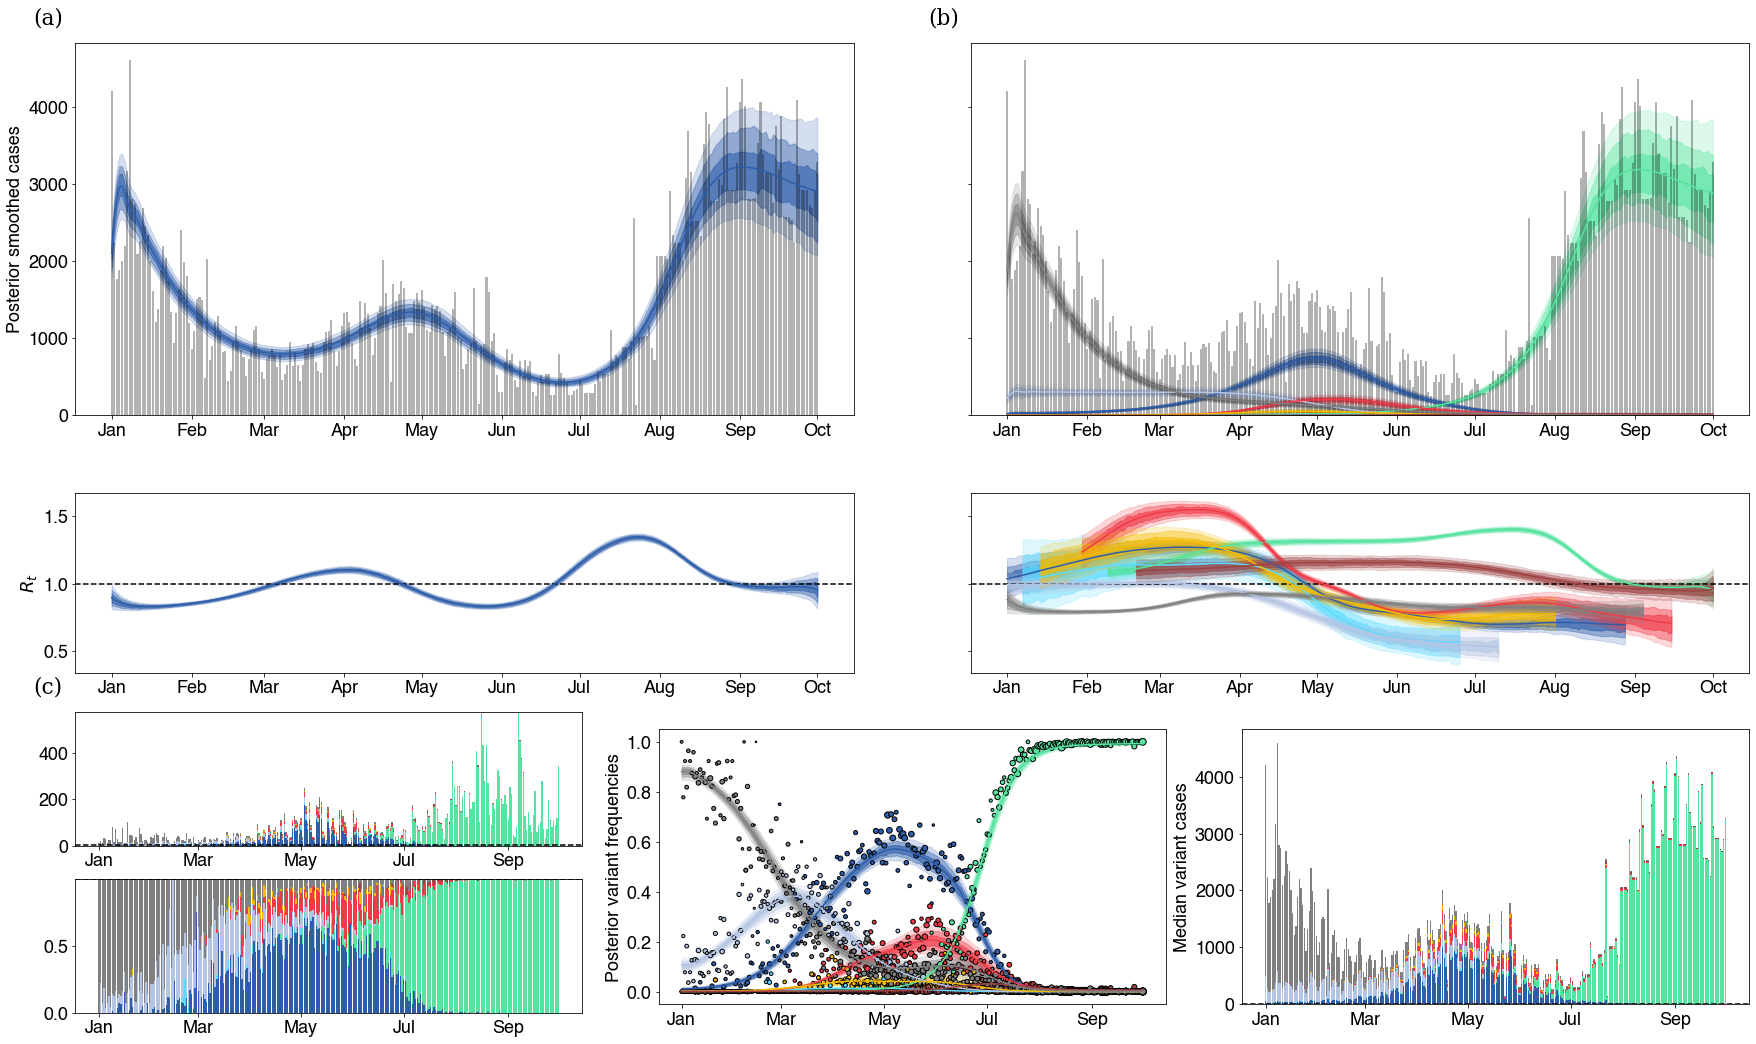
\includegraphics[width=\linewidth]{figs/fig_1.png}
  \caption{ (a) When assessing epidemic growth rates, we often compute a single effective reproduction number trajectory which is effectively an average over the all viruses in population.
    (b) Epidemics are made of different variants which may differ in fitness. Using case counts alongside sequences of different lineages allows us to understand the proportion of different variants in the population.
(c) Using both case count and frequency data, we can estimate the effective reproduction numbers of different lineages.}%
  \label{fig:1}
\end{figure}

%TODO: The labeling on this one will be made consistent with 1 and 3
\begin{figure}
  \centering
  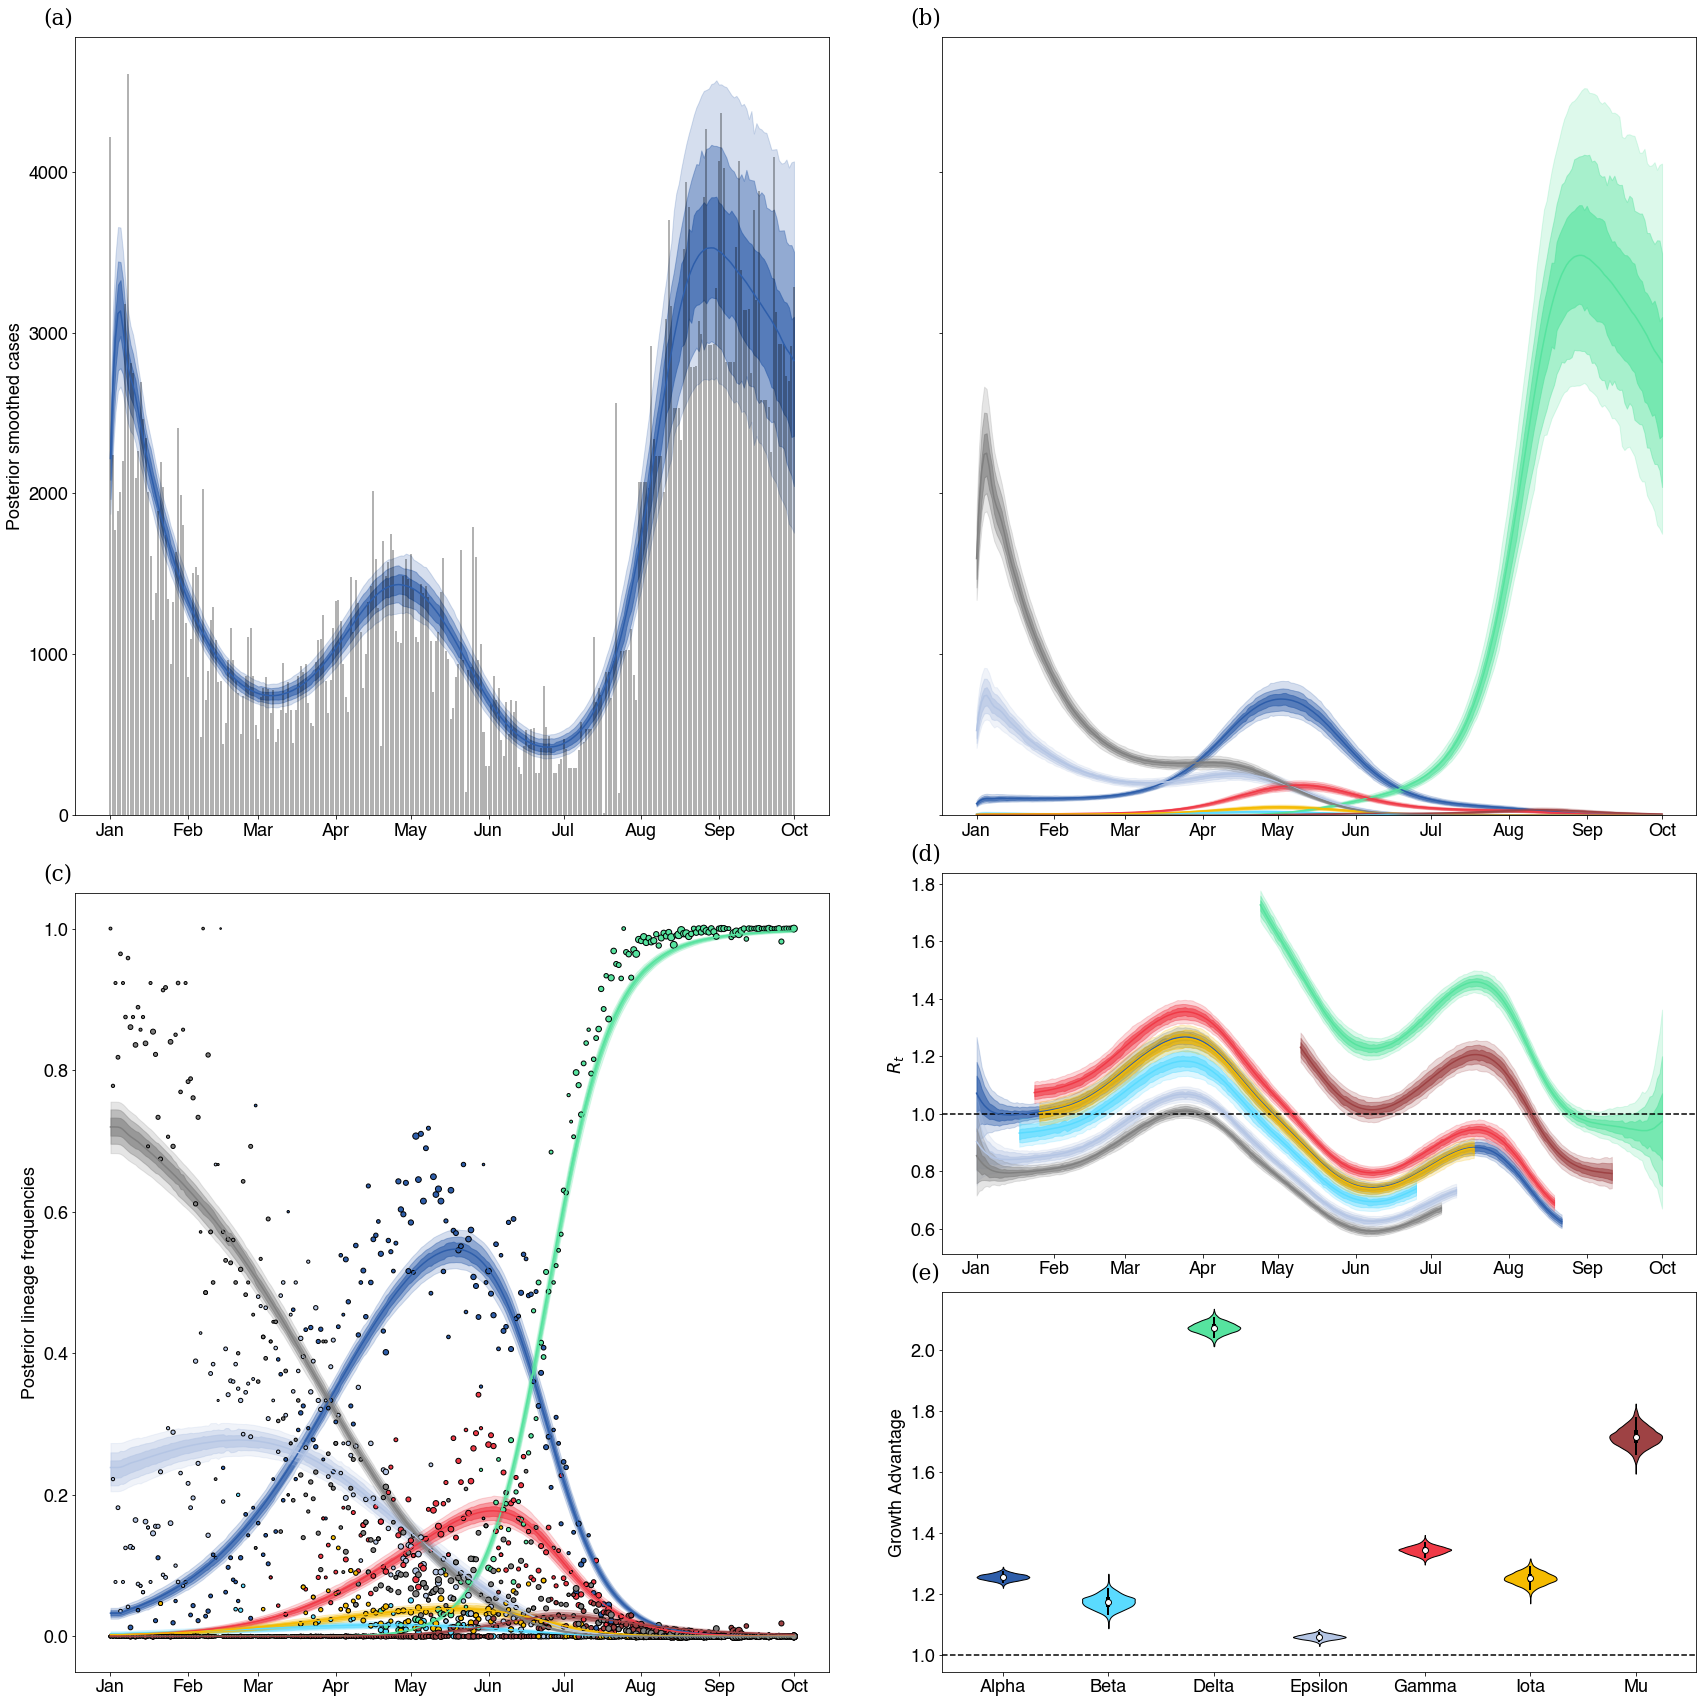
\includegraphics[width=\linewidth]{figs/fig_2_Washington.png}
  \caption{Fitting the fixed growth advantage model to Washington state data.
  (a) Posterior expected cases without weekly seasonality in reporting rate.
  (b) Posterior expected cases by lineage.
  (c) Posterior lineage frequency against observed sample frequency.
  (d) Lineage-specific effective reproduction number.
  (e) Posterior growth advantage by variant.}%
  \label{fig:2}
\end{figure}

\begin{figure}
  \centering
  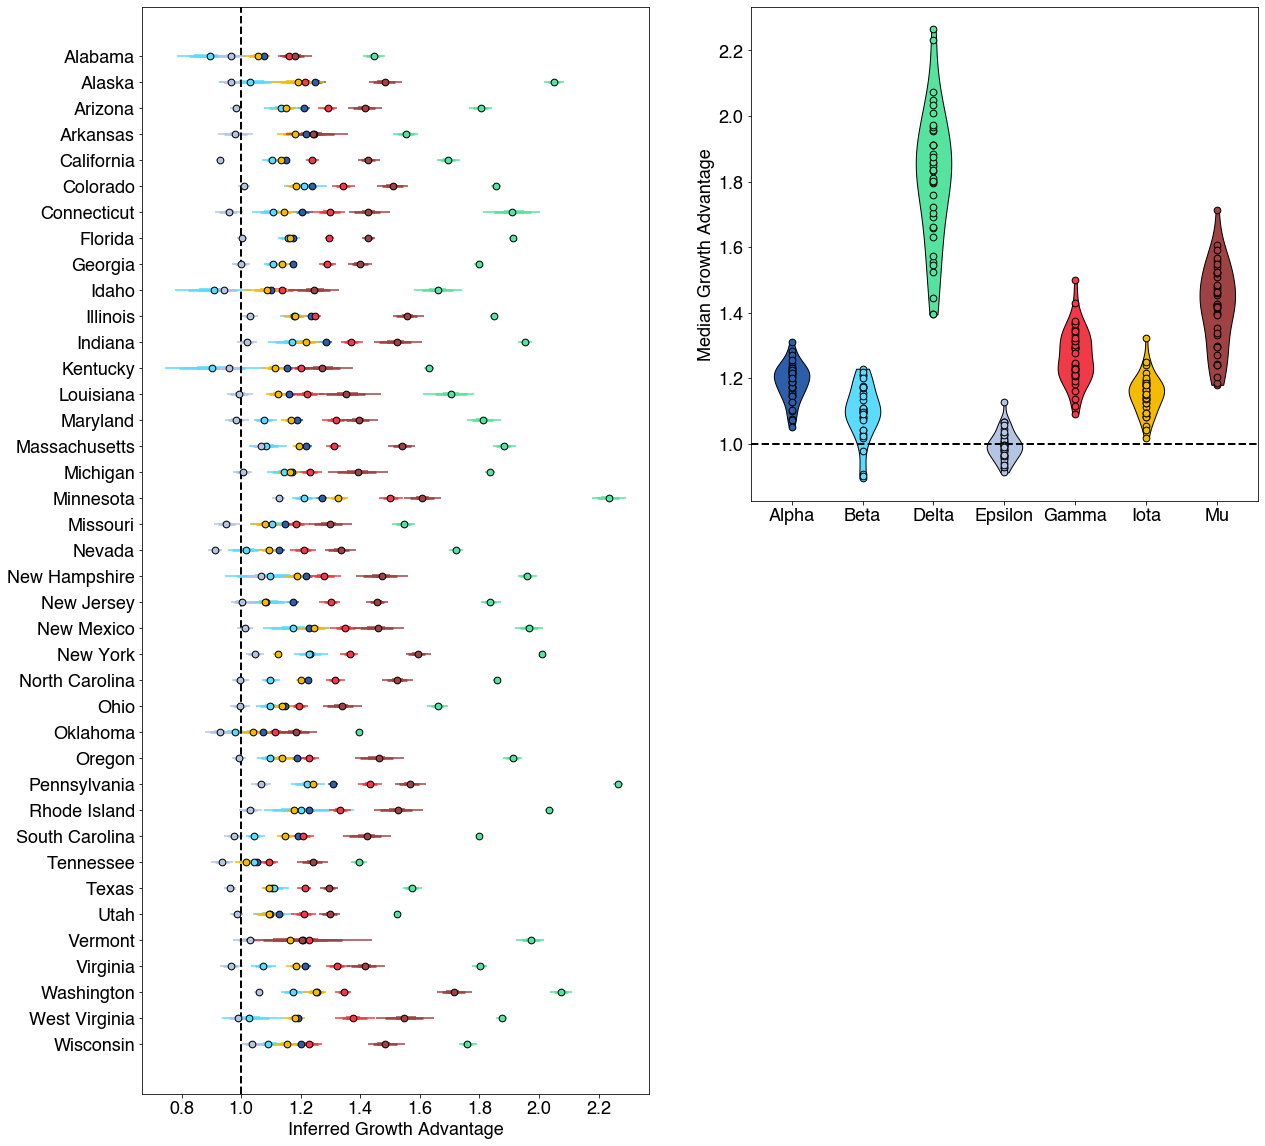
\includegraphics[width=\linewidth]{figs/fig_3_growth_advantages.png}
  \caption{Using structured model, we infer growth advantages for 7 variants in 46 US states.
  (a) State-wise growth advantages for variants of concern.
  (b) Same as (a) but visualized by variant.}%
  \label{fig:3}
\end{figure}

%TODO: Make more presentable
\begin{figure}
  \centering
  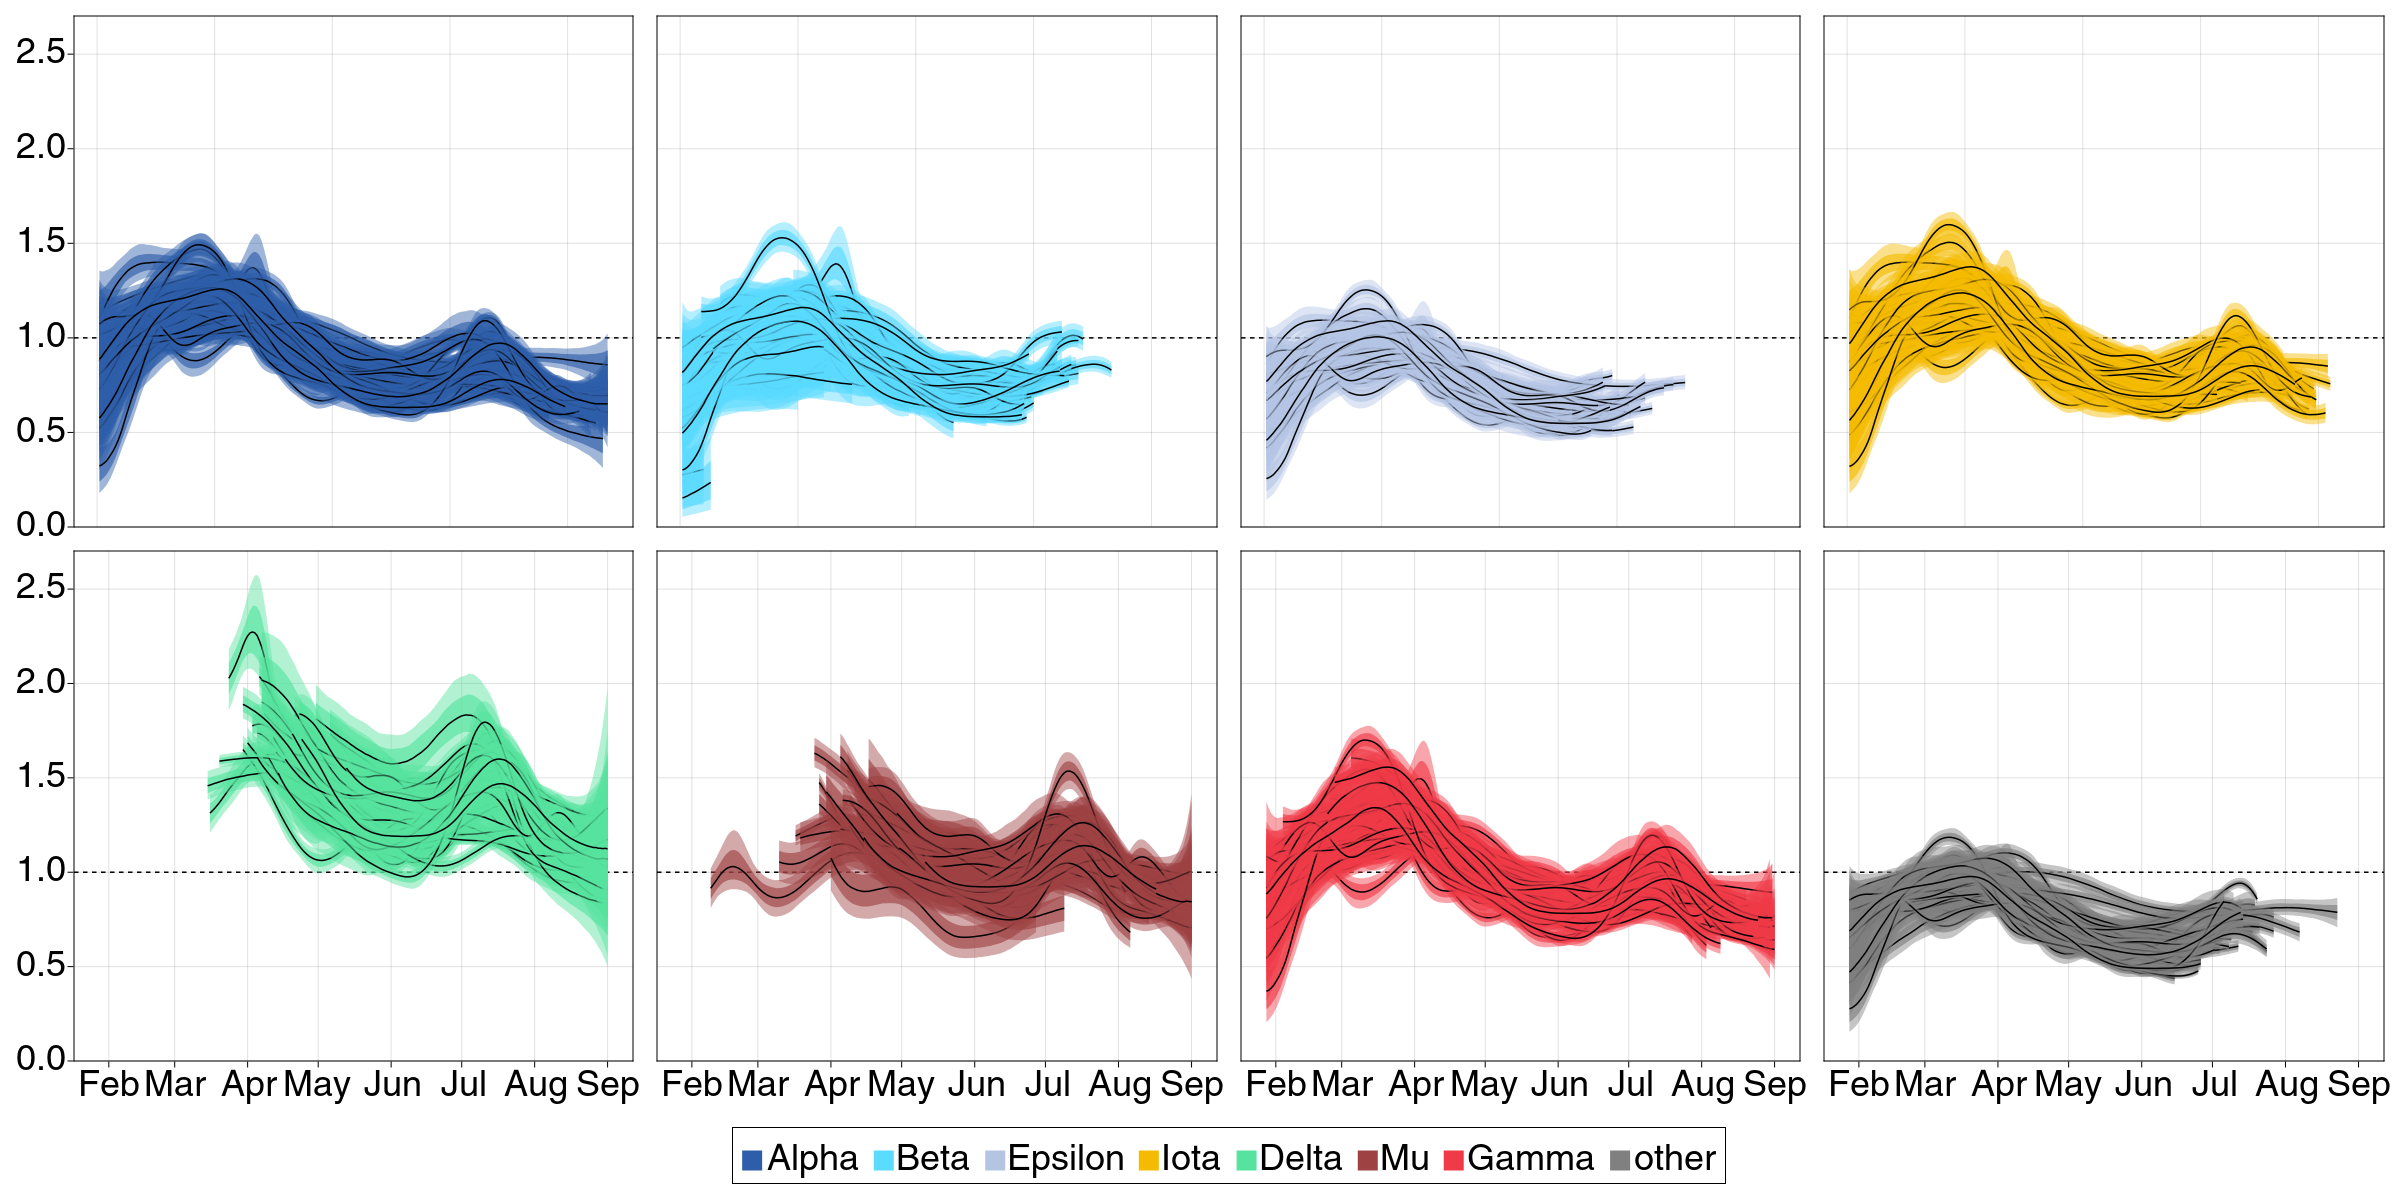
\includegraphics[width=\linewidth]{figs/fig_4_rt_consensus.png}
  \caption{Inferred effective reproduction numbers in 46 states show a consistent trend.}%
  \label{fig:4}
\end{figure}

%TODO: Make more presentable
\begin{figure}
  \centering
  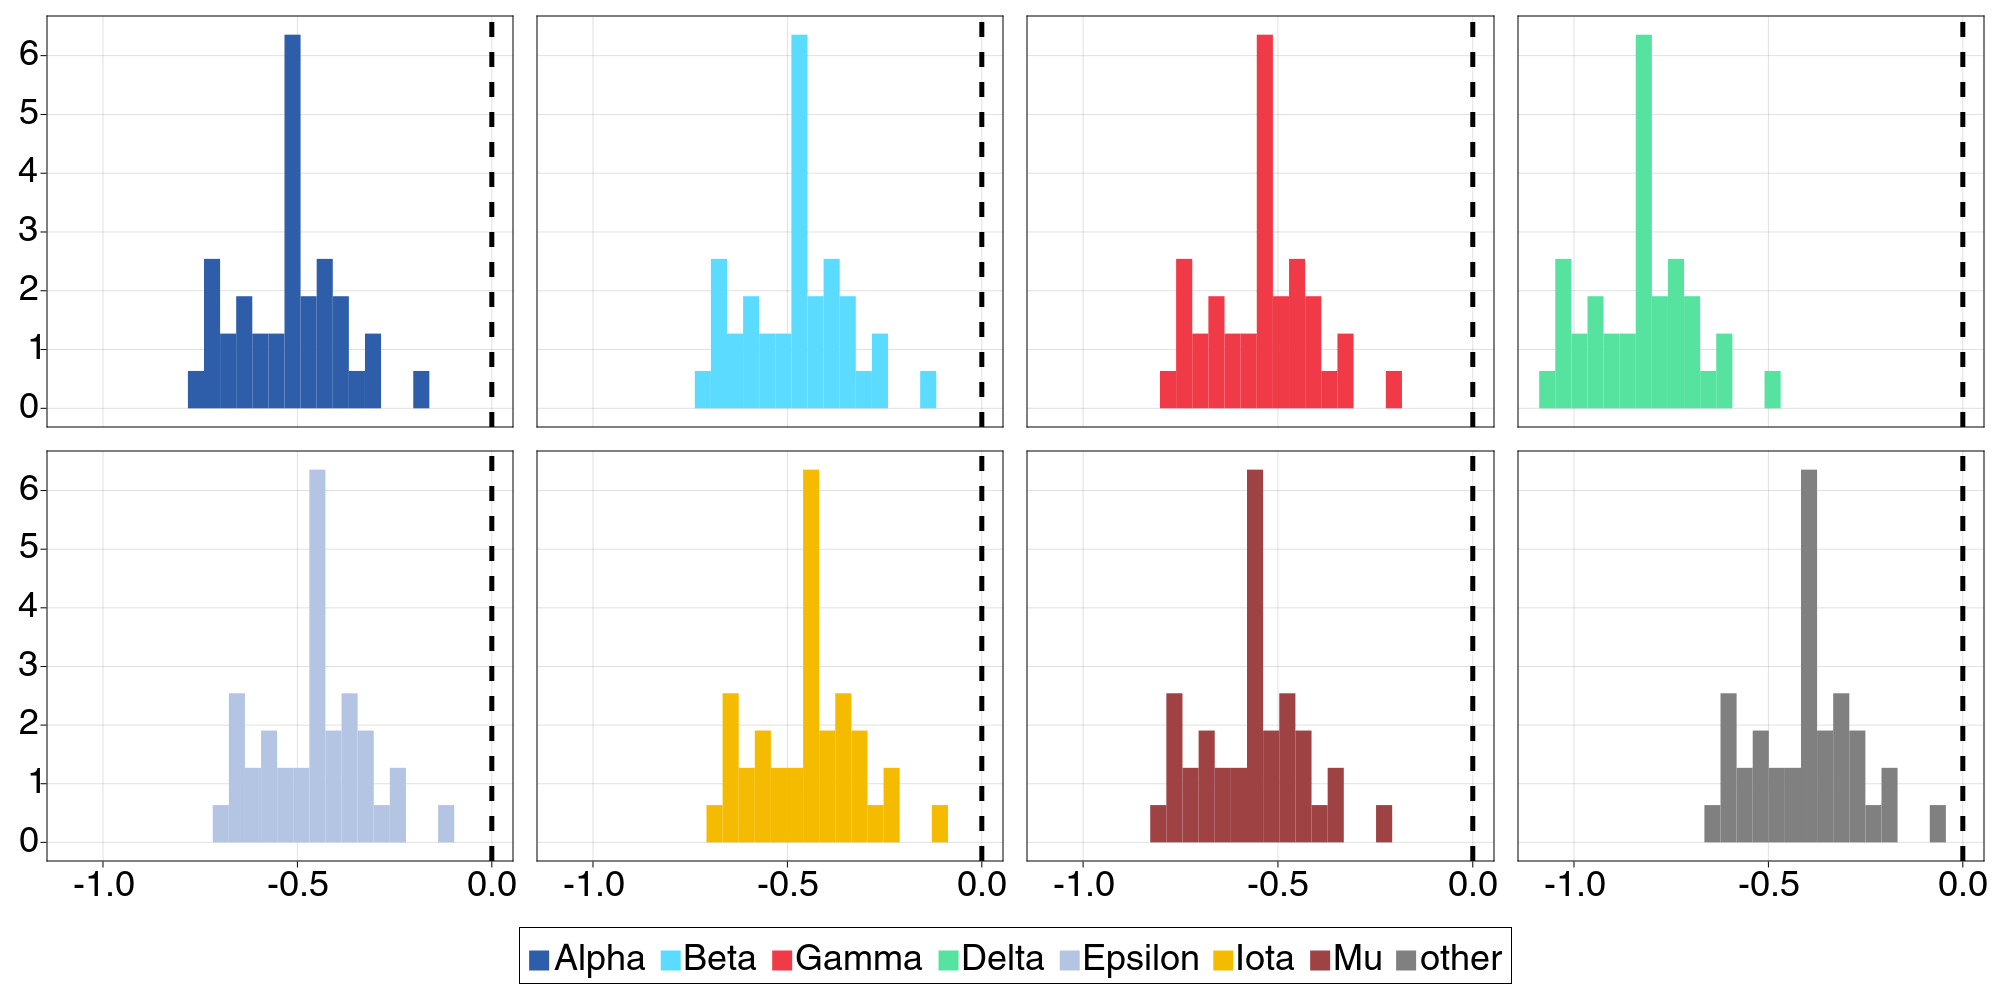
\includegraphics[width=\linewidth]{figs/fig_5_vaccination_effect.png}
  \caption{Estimated vaccination effect in various states.
  We see that vaccination decreases the effective reproduction number in all states and for all variants.}%
  \label{fig:5}
\end{figure}

\bibliographystyle{ieeetr}
\bibliography{rt-from-frequency-dynamics}

\newpage
\appendix

\section*{Supplemental Results}

\section{Relationship to multinomial logistic regression}

Other papers have tried to infer growth advantages of variants from sequence data alone, we show that the multinomial logistic regression model typically used in these analysis is roughly equivalent to our fixed growth advantage model but with additional restrictions on the generation time.
Multinomial logistic regression typically models the probability of a given observation belong to class $v$ as
\begin{equation}
  \text{Prob}(X = v) = f_{v} = \frac{p_{v}\exp(r_{v} t)}{\sum_{1\leq u\leq V} p_{u}\exp(r_{u} t)}.
\end{equation}
For our purpose, we can assume this probability is equivalent to the true frequency of variant $v$ in the population and in this case, $p_{v}$ is considered to be related to the prevalence on variant $v$ in the population at $t=0$ and $r_{v}$ can be considered to be the growth advantage relative to a pivot class $u_{*}$ which has $r_{k_{*}} = 1$.
In order to see the connection between this above model and ours, we return to the original renewal equation of the form
\begin{equation}
  I(t) = R_{t}\int_{0}^{t} I(t-\tau) g(\tau).
\end{equation}
Assuming that $g$  is a point mass at a mean generation time $T_{g}$, we have that
\begin{equation}
  I(nT_{g}) = \left(\prod_{i=1}^{n} R_{iT_{g}}\right) I(0).
\end{equation}
Assuming that there are several variants following these same dynamics, we have that the frequency of a given variant $v$ can be written as
\begin{equation}
  f_{v}(nT_{g}) = \frac{I_{v}(nT_{g})}{\sum_{1\leq u \leq V} I_{u}(nT_{g})}.
\end{equation}
If we assume a constant growth advantage as in our model, we then have that $R_{t,v} = \Delta_{v} R_{t}$, so that
\begin{equation}
  f_{v}(nT_{g}) =  \frac{\Delta_{v}^{n} I_{v}(0)}{\sum_{1\leq u \leq V} \Delta_{u}^{n} I_{u}(0)}.
\end{equation}
Writing $\Delta_{v} = \exp(\delta_{v})$ and $t = n T_{g}$, allows us to see that
\begin{equation}
  f_{v}(t) = \frac{I_{v}(0) \exp(\frac{\delta_{v}}{T_{g}} t)}{\sum_{1\leq u \leq V}I_{u}(0) \exp(\frac{\delta_{u}}{T_{g}} t)}.
\end{equation}
By fixing one pivot class so that $I_{u_{*}} = \delta_{u_{*}} / T_{g} = 1$, we can identify our model with the multinomial logistic regression by relating the parameters as

\begin{align}
  \delta_{v} &= r_{v}T_{g}\\
  I_{v}(0) &= p_{v}.
\end{align}

This shows that the multinomial logistic regression functions similarly to our fixed growth advantage model except with the additional assumption that the generation time is a point mass at $T_{g}$.
This assumption additionally allows us to relate the epidemic growth rate $r$ and the effective reproduction number as $R = \exp(r T_{g})$ \cite{Wallinga2006}.
Further work is needed to directly quantify how making this assumption on the generation time affects the inferred growth advantages.

\begin{figure}
  \centering
  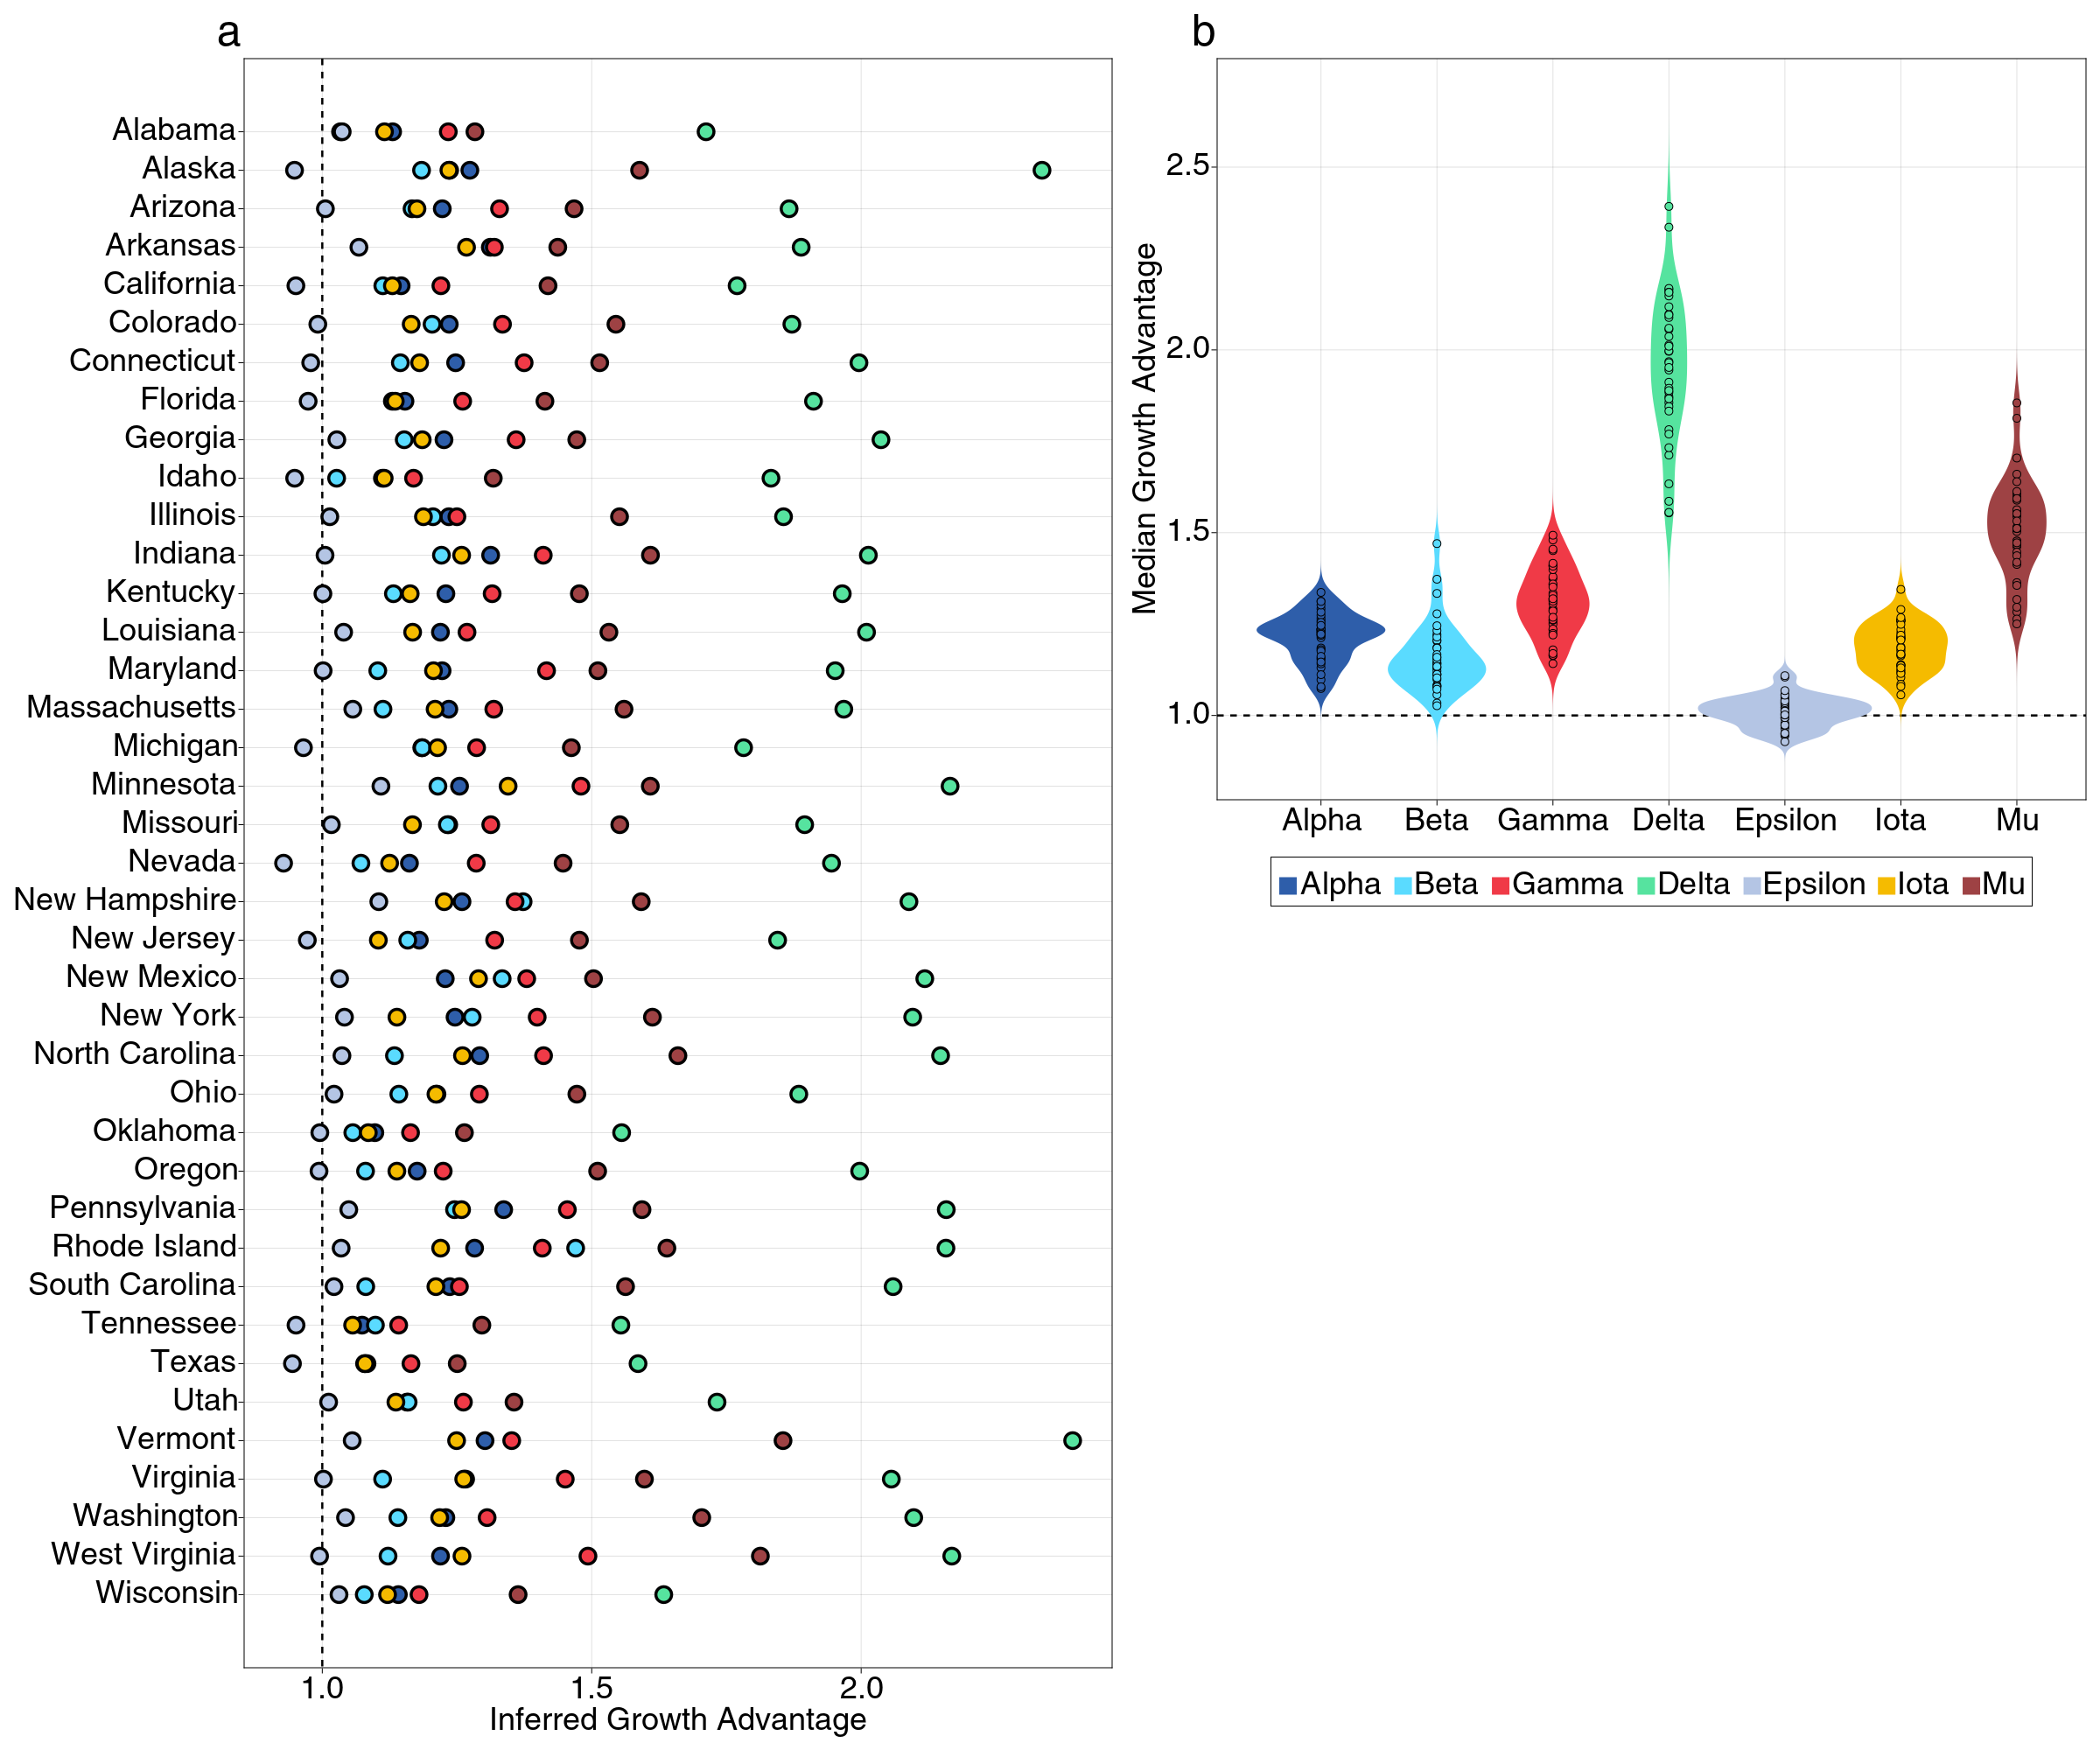
\includegraphics[width=\linewidth]{figs/fig_MLR_growth_advantages_supp.png}
  \caption{Assess growth advantages in various states using Multinomial Logistic Regression model assuming generation time $T_{g} = 5.2$.
  (a) Growth advantages visualized by state.
  (b) Same as (a) but grouped by variant.}%
  \label{fig:MLR_growth_advantages}
\end{figure}

%TODO: Any other supplemental sections necessary?

%TODO: Supplemental version of fig 2 for different states
%TODO: Might want to include posterior predictive of observed sequences of each variant type.

\end{document}
